\stepcounter{section}
\section*{\Large\centering {CHAPTER 4 \\ SYSTEM DESIGN}}
\addcontentsline{toc}{section}{CHAPTER 4: System Design}\label{4}
\subsection{Design}
\begin{enumerate}[label=\roman*.]
    \item \textbf{Class Diagram}
          \begin{center}
              \begin{figure}[H]
                  \centering
                  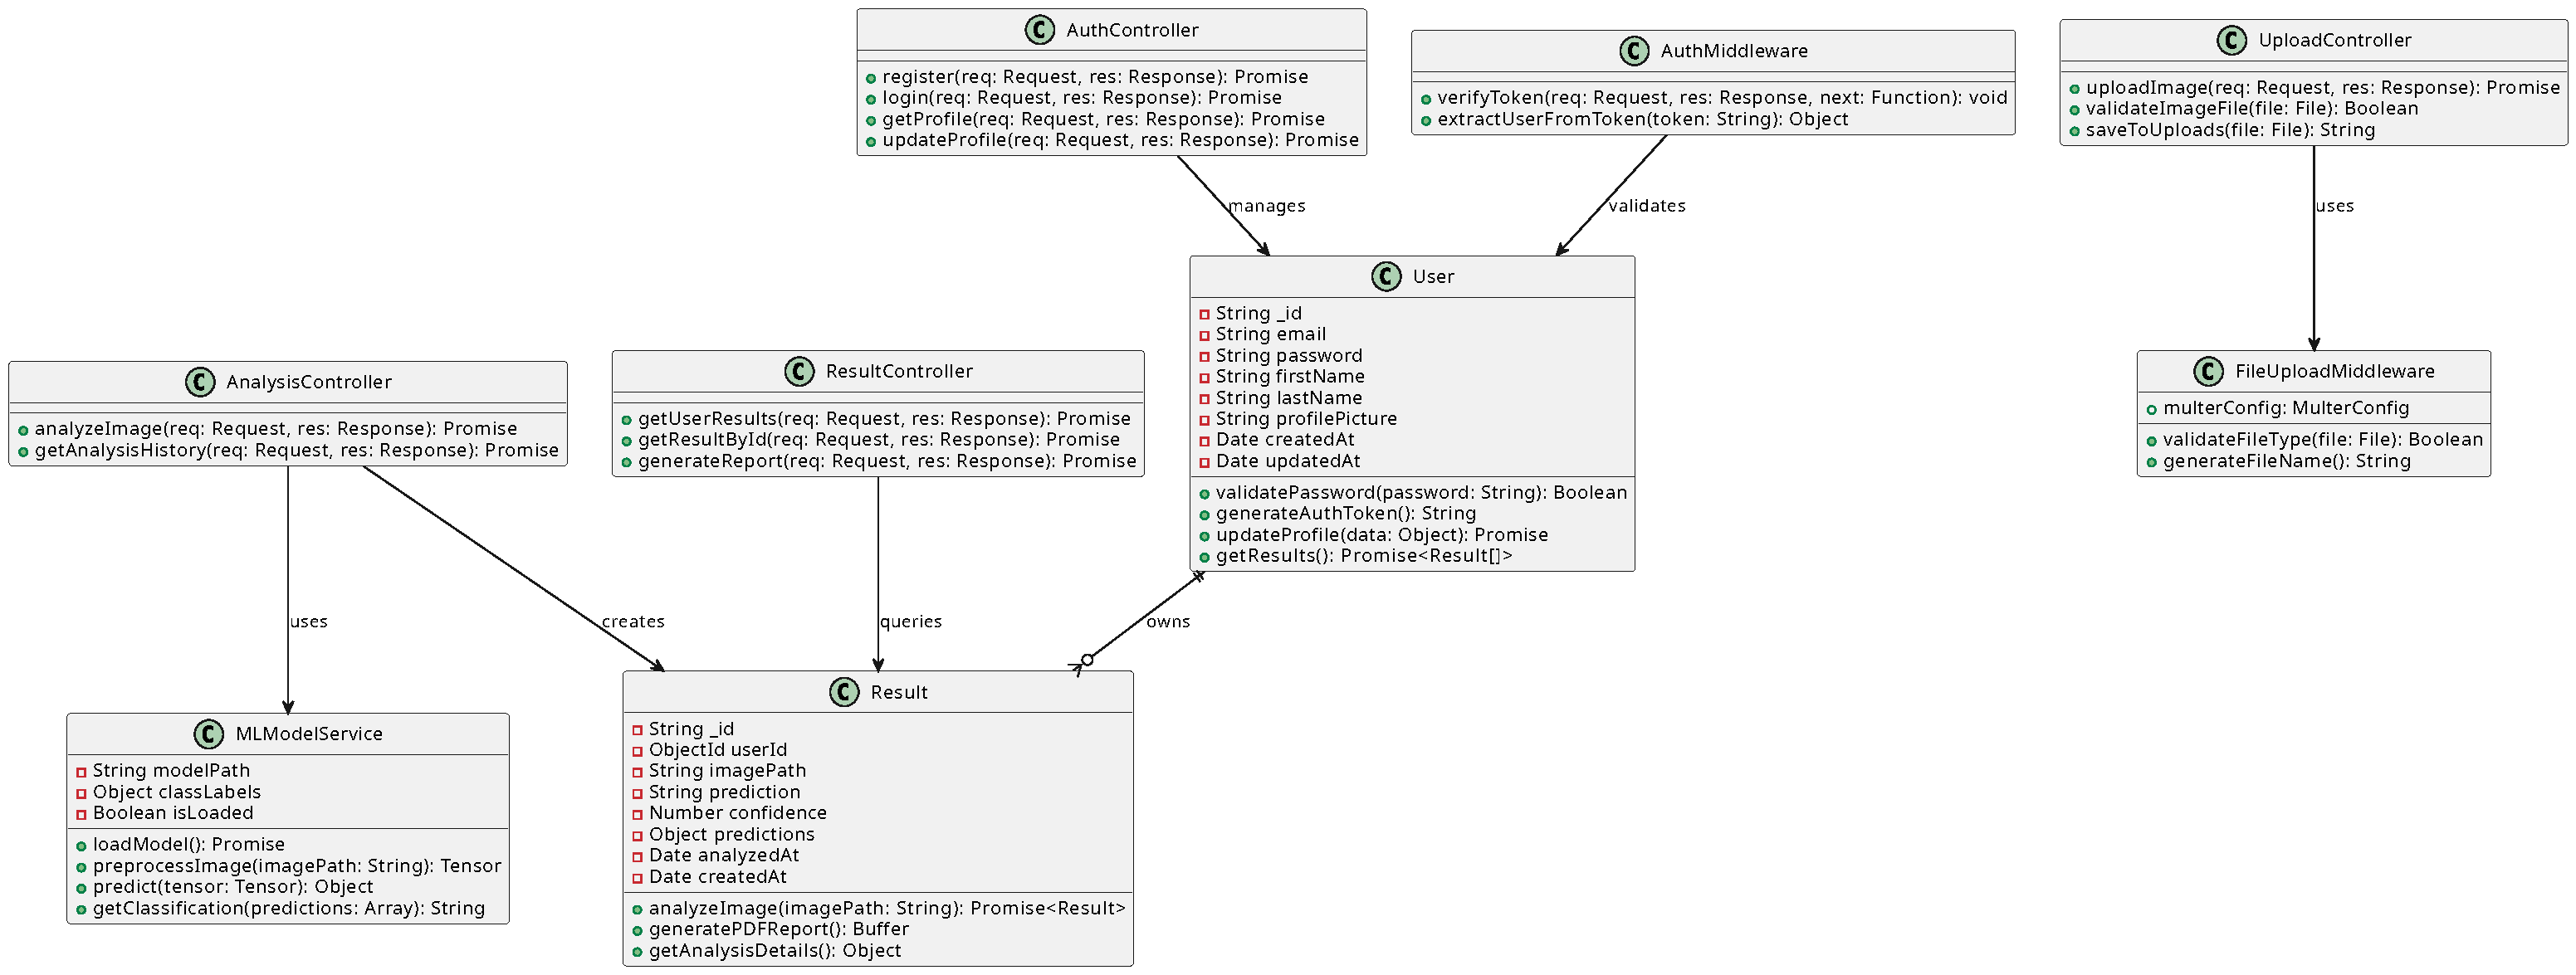
\includegraphics[width=1\linewidth]{Images/Refined/class.pdf}
                  \caption{Refinement of Class Diagram}
                  \label{fig:RefinementofClassDiagram}
              \end{figure}
          \end{center}
          The refined class diagram significantly expands upon the high-level version by introducing detailed implementation specifics and architectural components. While the original diagram focused on core domain entities, this version incorporates the complete MVC architecture with dedicated controller classes for different functional areas. The AuthController, UploadController, AnalysisController, and ResultController represent the application's API endpoints and business logic handlers. New middleware components like AuthMiddleware and FileUploadMiddleware demonstrate the request processing pipeline and security layers. The MLModelService class provides more granular methods for model loading, image preprocessing, tensor operations, and classification logic. Database models now include private fields with proper encapsulation and detailed method signatures showing parameter types and return values. This refined diagram reveals the actual software architecture with separation of concerns, dependency injection patterns, and proper abstraction layers that weren't visible in the high-level overview.
          \newpage
    \item \textbf{Object Diagram}
          \begin{center}
              \begin{figure}[H]
                  \centering
                  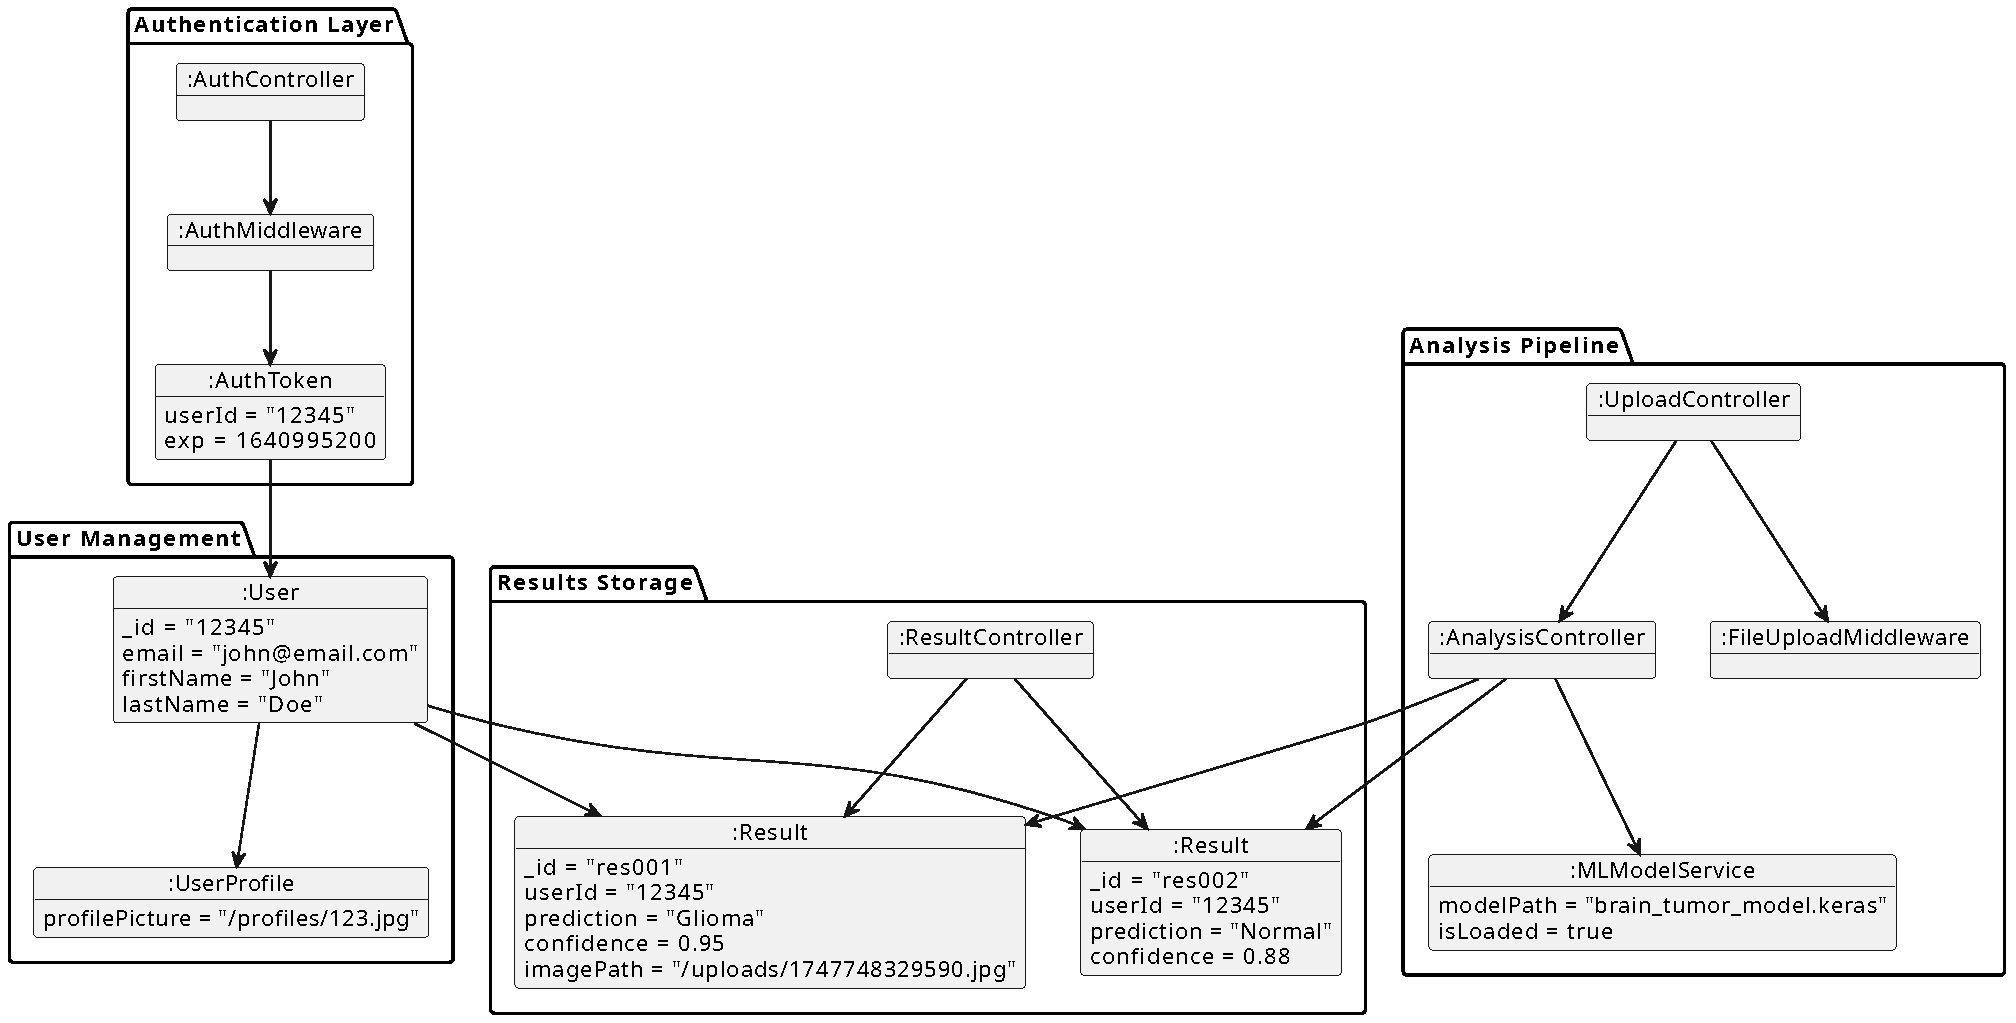
\includegraphics[width=1\linewidth]{Images/Refined/obj.pdf}
                  \caption{Refinement of Object Diagram}
                  \label{fig:RefinementofObjectDiagram}
              \end{figure}
          \end{center}
          The refined object diagram presents a more comprehensive runtime view by organizing components into logical packages representing different architectural layers. Unlike the simple high-level version, this diagram shows the Authentication Layer with controller instances, middleware objects, and JWT token representations. The User Management package demonstrates the relationship between user entities and their profile information. The Analysis Pipeline package reveals the complete request processing flow from upload controllers through file middleware to ML services. The Results Storage package shows how multiple result instances are managed by dedicated controllers. This detailed view exposes the actual object collaboration patterns, package dependencies, and layer interactions that occur during system execution, providing insights into the implementation architecture that the high-level diagram abstracted away.

    \item \textbf{State Diagram}
          \begin{center}
              \begin{figure}[H]
                  \centering
                  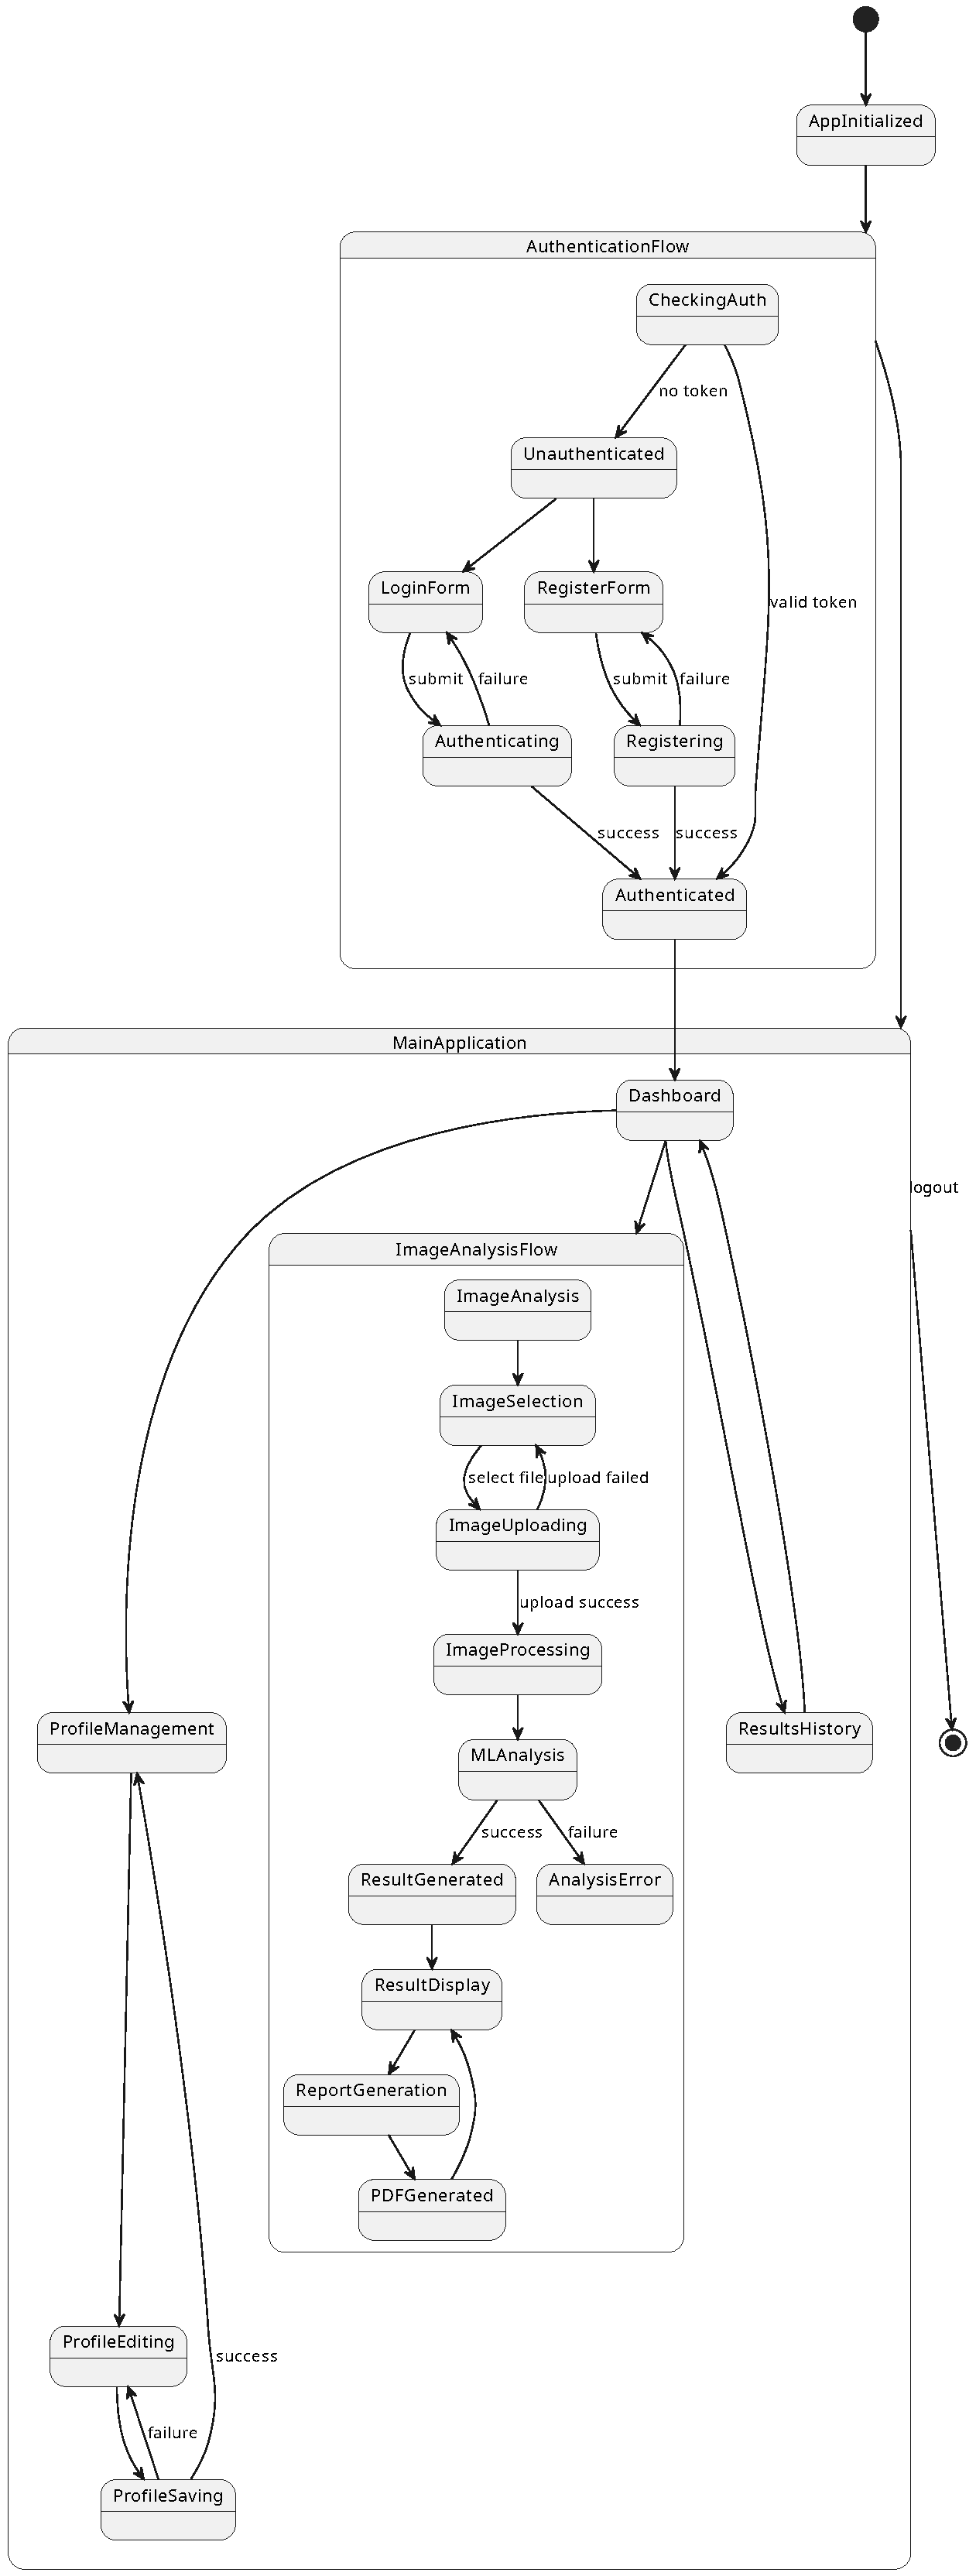
\includegraphics[width=0.6\linewidth]{Images/Refined/state.pdf}
                  \caption{Refinement of State Diagram}
                  \label{fig:RefinementofStateDiagram}
              \end{figure}
          \end{center}
          The refined state diagram transforms the simple linear workflow into a comprehensive state machine with nested states and complex transitions. The original diagram showed basic authentication and analysis states, while this version introduces hierarchical state organization with distinct flows for authentication, image analysis, and profile management. The AuthenticationFlow composite state includes detailed substates for token checking, form validation, and error handling. The ImageAnalysisFlow demonstrates the complete image processing pipeline with states for selection, uploading, processing, ML analysis, result generation, and error recovery. Additional states for profile management and report generation show parallel user workflows. This refined diagram captures real-world application complexity with multiple concurrent processes, error states, and recovery mechanisms that provide a complete picture of system behavior under various conditions.
    \item \textbf{Sequence Diagram}
          \begin{center}
              \begin{figure}[H]
                  \centering
                  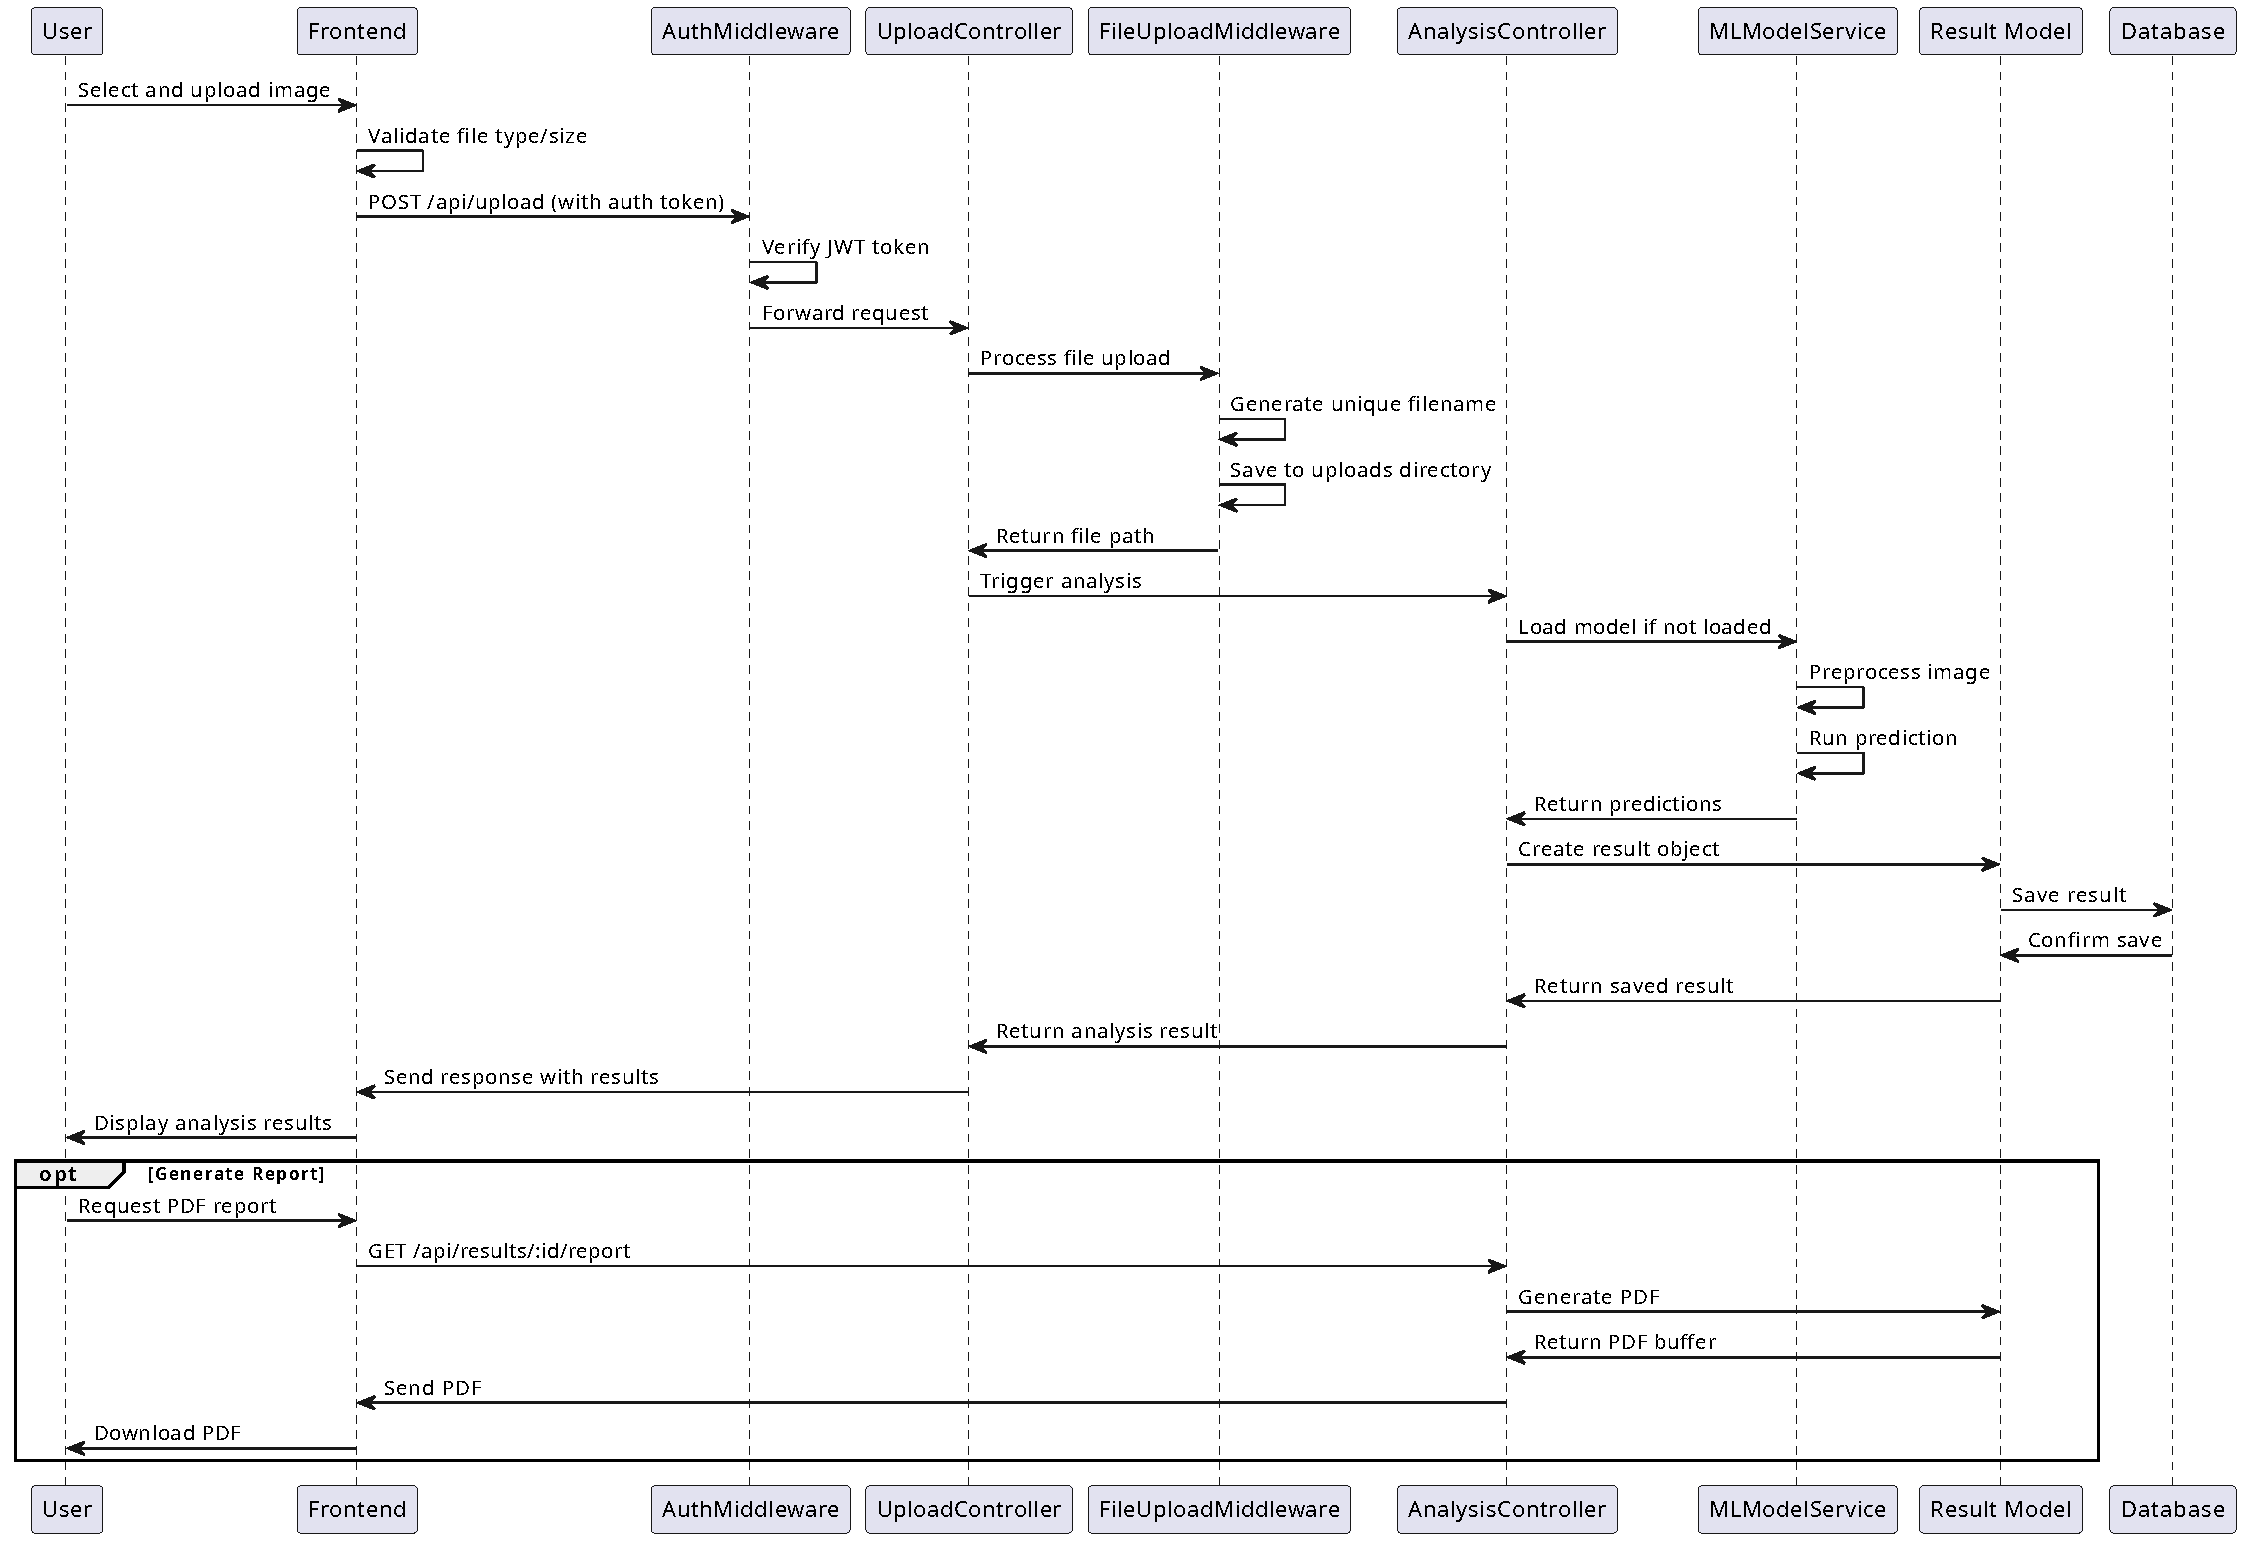
\includegraphics[width=1\linewidth]{Images/Refined/sequence.pdf}
                  \caption{Refinement of Sequence Diagram}
                  \label{fig:RefinementofSequenceDiagram}
              \end{figure}
          \end{center}
          The refined sequence diagram expands the simple high-level interaction into a detailed multi-participant collaboration showing the complete request processing pipeline. While the original diagram showed basic frontend-backend-model communication, this version reveals the actual middleware stack, authentication verification, file processing layers, and database operations. The diagram now includes AuthMiddleware for token verification, FileUploadMiddleware for file handling, and separate controllers for different responsibilities. Additional detail shows model loading optimization, image preprocessing steps, database confirmation patterns, and optional PDF generation workflows. Error handling scenarios and alternative flows are represented through optional fragments. This comprehensive view demonstrates the actual software architecture with proper separation of concerns, middleware processing, and the complete data transformation pipeline from user input to final output.

    \item \textbf{Activity Diagram}
          \begin{center}
              \begin{figure}[H]
                  \centering
                  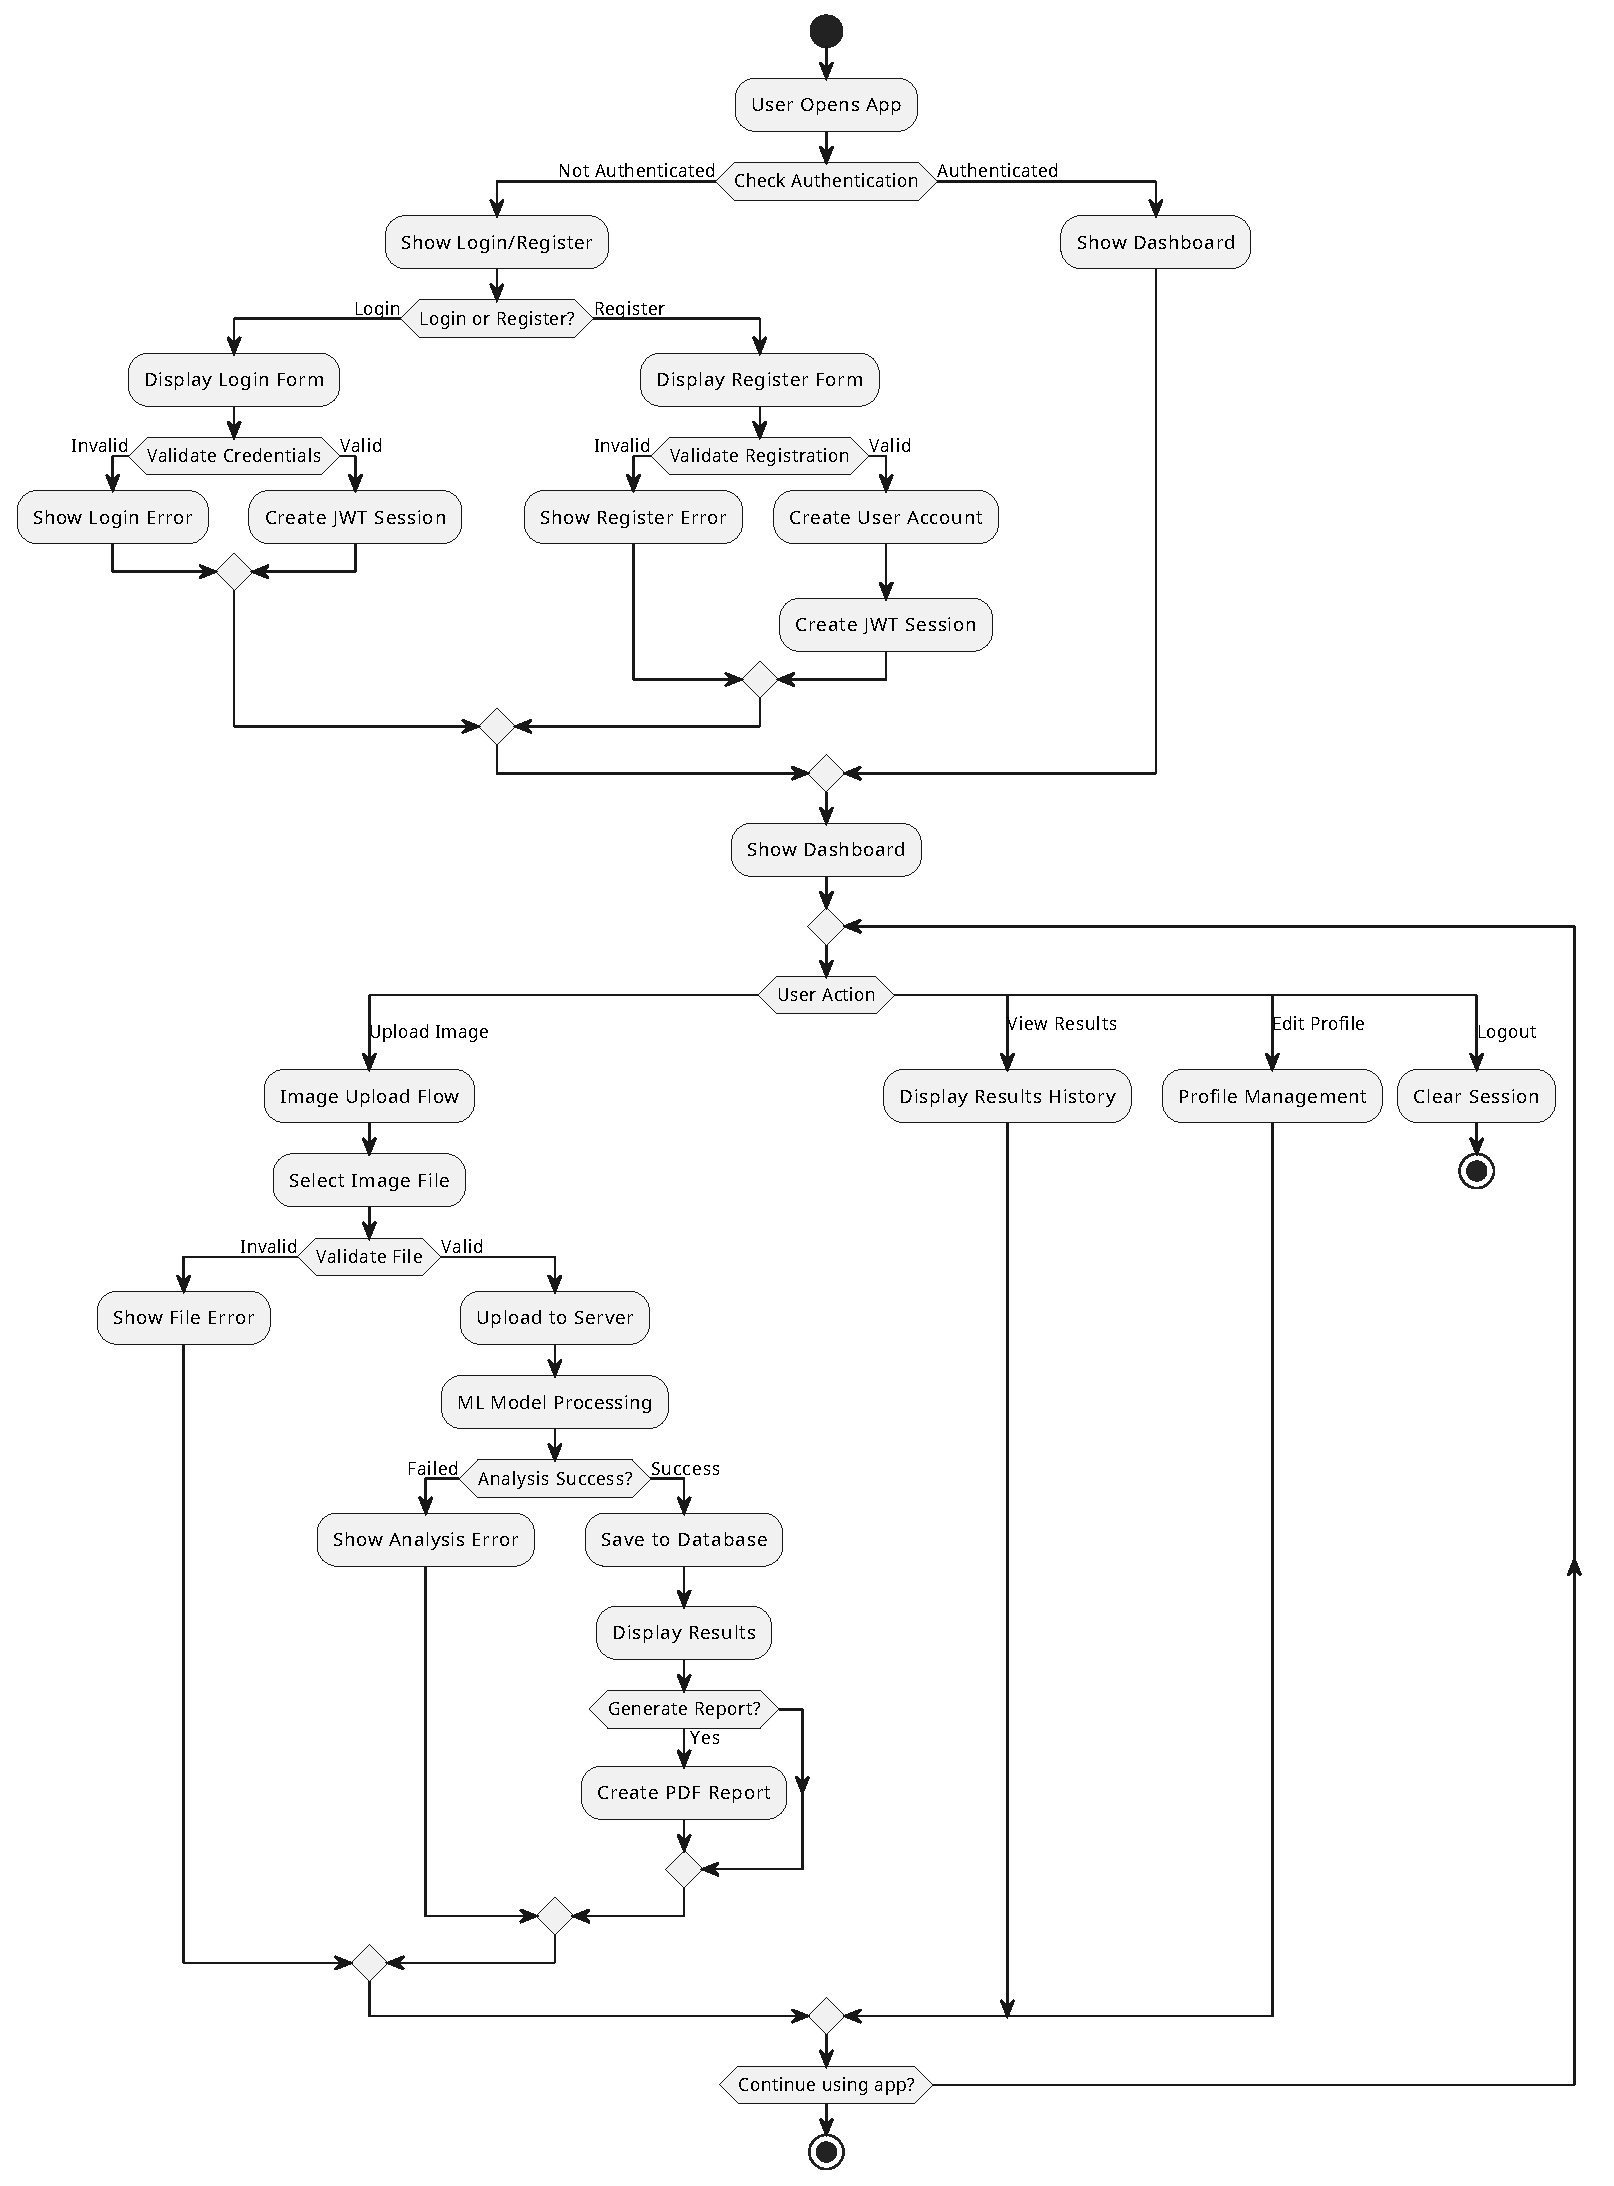
\includegraphics[width=0.8\linewidth]{Images/Refined/activity.pdf}
                  \caption{Refinement of Activity Diagram}
                  \label{fig:RefinementofActivityDiagram}
              \end{figure}
          \end{center}
          The refined activity diagram transforms the basic decision flow into a comprehensive business process model with detailed error handling and multiple workflow branches. The high-level diagram showed simple authentication and analysis paths, while this version incorporates complete user registration flows, detailed validation processes, and comprehensive error recovery mechanisms. New branches handle user account creation, profile management workflows, and multiple analysis result viewing options. The diagram now shows parallel processes for different user actions, detailed file validation steps, and granular ML processing phases. Error states are properly connected to recovery paths, and the workflow includes session management, logout procedures, and application lifecycle management. This detailed process model reflects the actual user experience with all possible paths, decision points, and system responses that users encounter during real application usage.
    \item \textbf{Component Diagram}
          \begin{center}
              \begin{figure}[H]
                  \centering
                  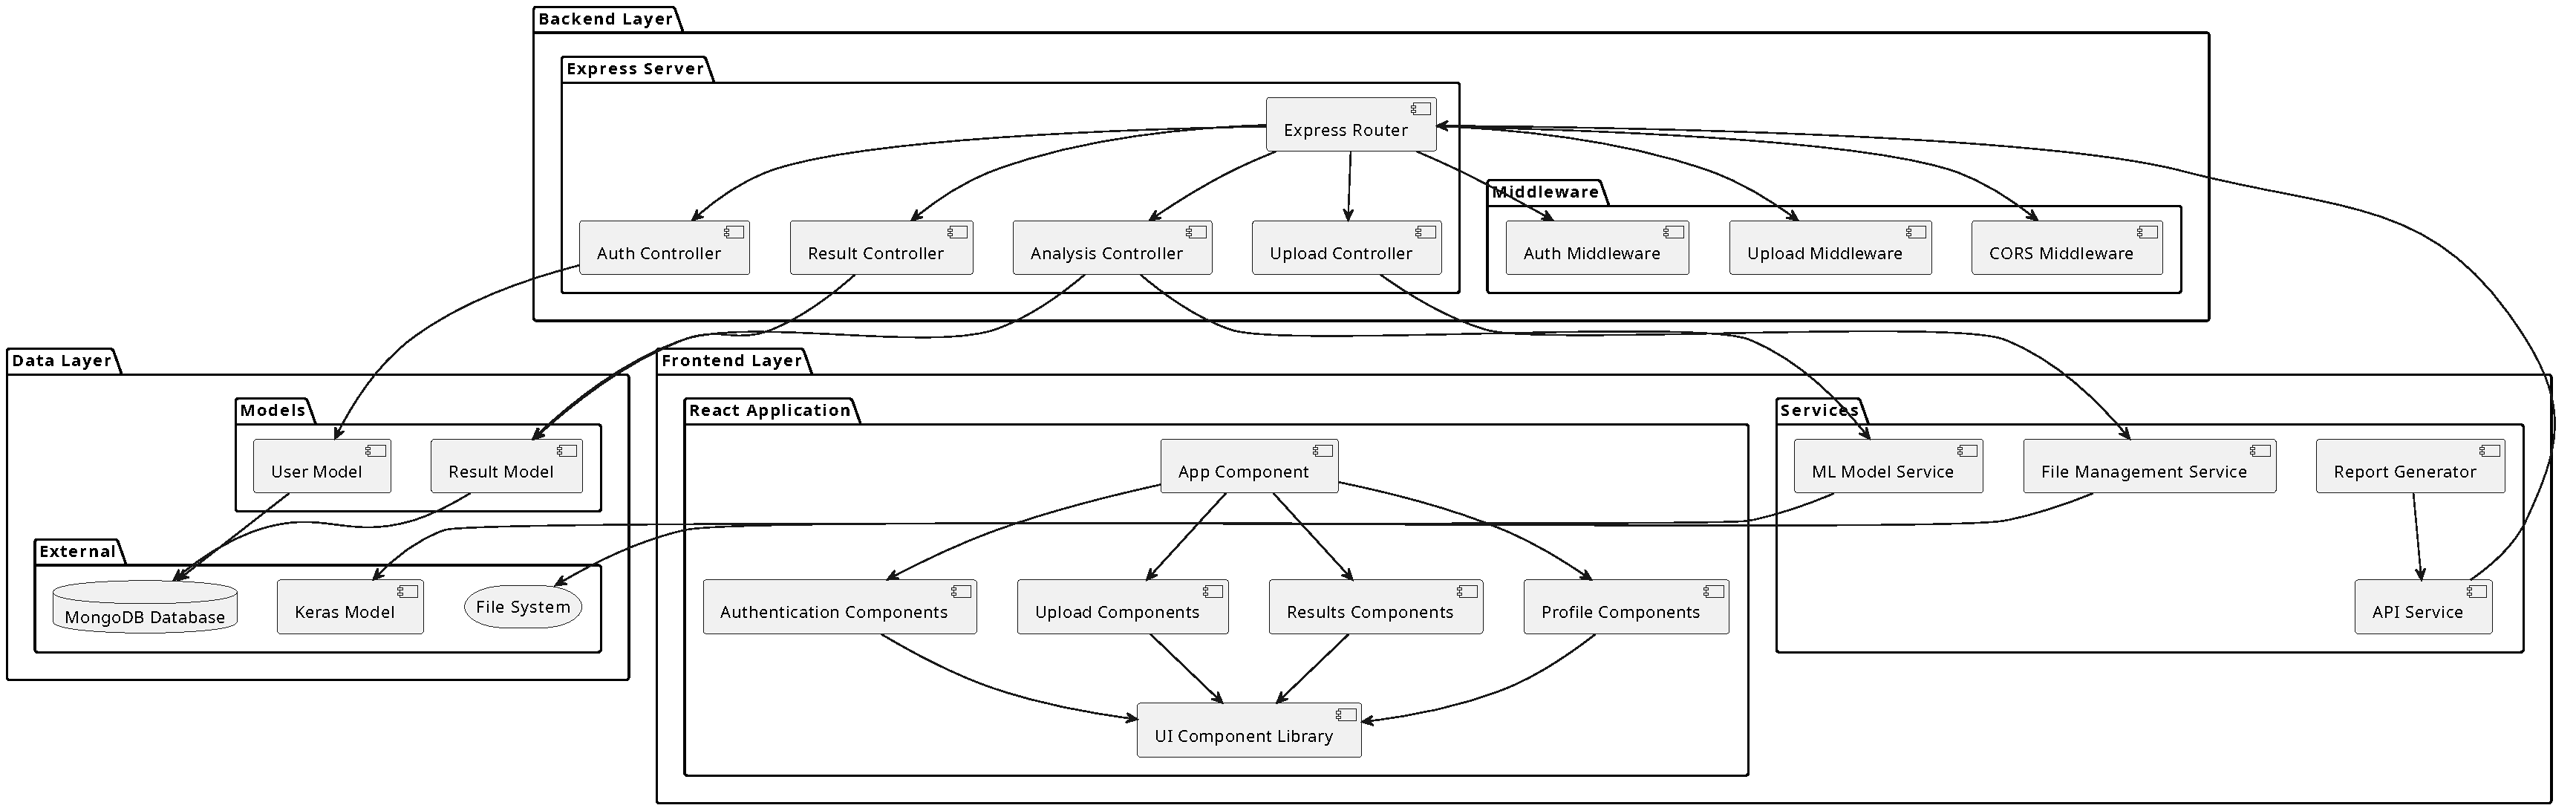
\includegraphics[width=1\linewidth]{Images/Refined/component.pdf}
                  \caption{Refinement of Component Diagram}
                  \label{fig:RefinementofComponentDiagram}
              \end{figure}
          \end{center}
          The component diagram presents the system's architectural organization across three distinct layers, demonstrating how components collaborate to deliver application functionality. The Frontend Layer contains the React application with its constituent components for authentication, file upload, results display, and profile management, all built upon a shared UI component library. The API Service and Report Generator provide client-side services for server communication and document generation. The Backend Layer implements the Express server architecture with route handlers, controllers for different functional domains, and middleware components for cross-cutting concerns like authentication, file upload processing, and CORS handling. Business logic services handle ML model operations and file management. The Data Layer abstracts database operations through Mongoose models while connecting to external systems including MongoDB for data persistence, the file system for image storage, and the Keras model for machine learning predictions. This organization demonstrates clear separation of concerns with defined interfaces between layers.
          \newpage
    \item \textbf{Deployment Diagram}
          \begin{center}
              \begin{figure}[H]
                  \centering
                  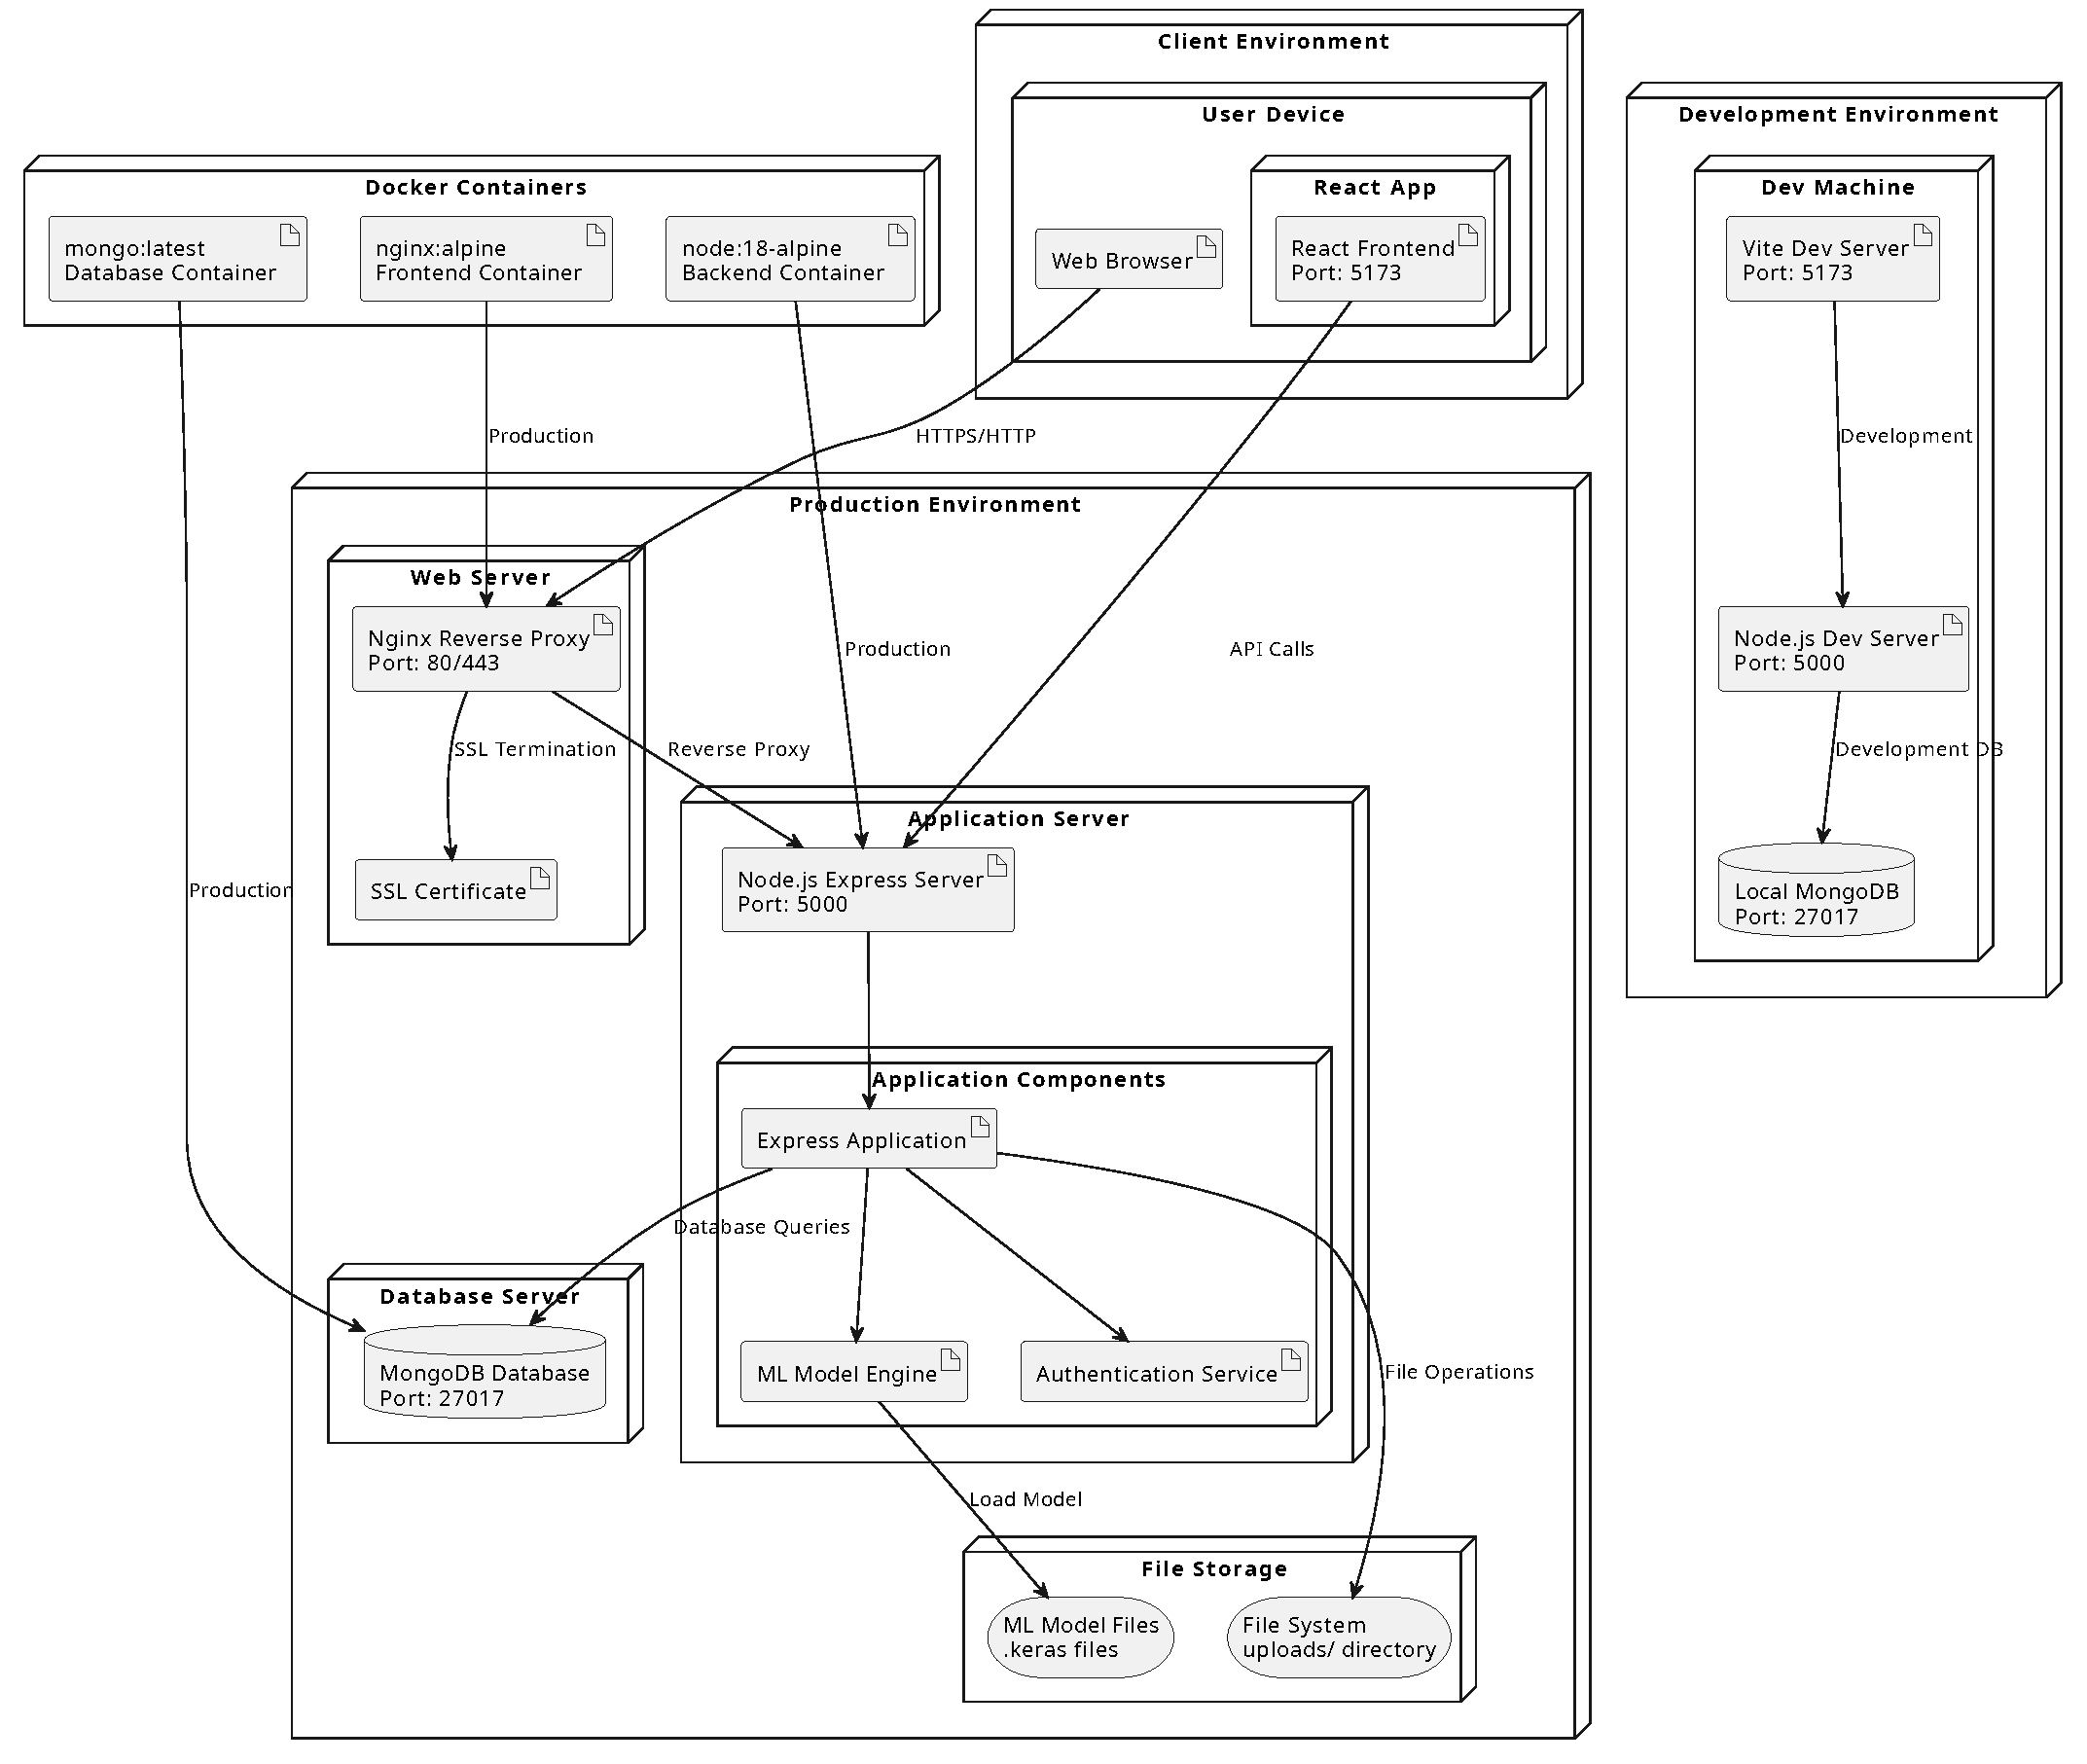
\includegraphics[width=1\linewidth]{Images/Refined/deployment.pdf}
                  \caption{Refinement of Deployment Diagram}
                  \label{fig:RefinementofDeploymentDiagram}
              \end{figure}
          \end{center}
          The deployment diagram illustrates the complete system infrastructure across development, production, and containerized environments. The Client Environment shows end-user devices running web browsers that host the React frontend application. The Production Environment demonstrates a multi-tier architecture with Nginx serving as a reverse proxy and SSL termination point, forwarding requests to the Node.js application server. The application server hosts the Express framework with integrated ML model engine and authentication services, connecting to a dedicated MongoDB database server and file storage systems for uploads and model files. The Development Environment mirrors production with local development servers and database instances for testing. Docker containerization provides deployment flexibility with separate containers for frontend, backend, and database components. This infrastructure supports scalability, security, and maintainability while providing development-production parity through containerized deployments that ensure consistent environments across different deployment targets.
\end{enumerate}

\subsection{Algorithm Details}
\textbf{Convolutional Neural Network (\gls{cnn})}

A \gls{cnn} is a type of artificial neural network specifically designed for
processing and classifying visual data. In this project, we developed a custom
\gls{cnn} architecture tailored for medical imaging.

The primary algorithm powering the brain tumor detection system is a
Convolutional Neural Network implemented using TensorFlow/Keras framework. This
deep learning algorithm employs multiple convolutional layers with ReLU
activation functions, pooling layers for dimensionality reduction, and fully
connected dense layers for final classification~\cite{krizhevsky2012imagenet}.
The CNN automatically learns hierarchical features from brain MRI images,
starting with simple edge detection in early layers and progressing to complex
anatomical structures in deeper layers. The network architecture includes batch
normalization for training stability~\cite{ioffe2015batch}, dropout layers for
regularization to prevent overfitting~\cite{srivastava2014dropout}, and a
softmax output layer that produces probability distributions across four
classes: Glioma, Meningioma, Pituitary tumors, and Normal brain scans. The
algorithm processes 224$ \times$ 224 pixel RGB images and outputs confidence
scores for each tumor category, enabling medical professionals to assess the
reliability of predictions alongside the primary classification result.

\begin{figure}[H]
    \centering
    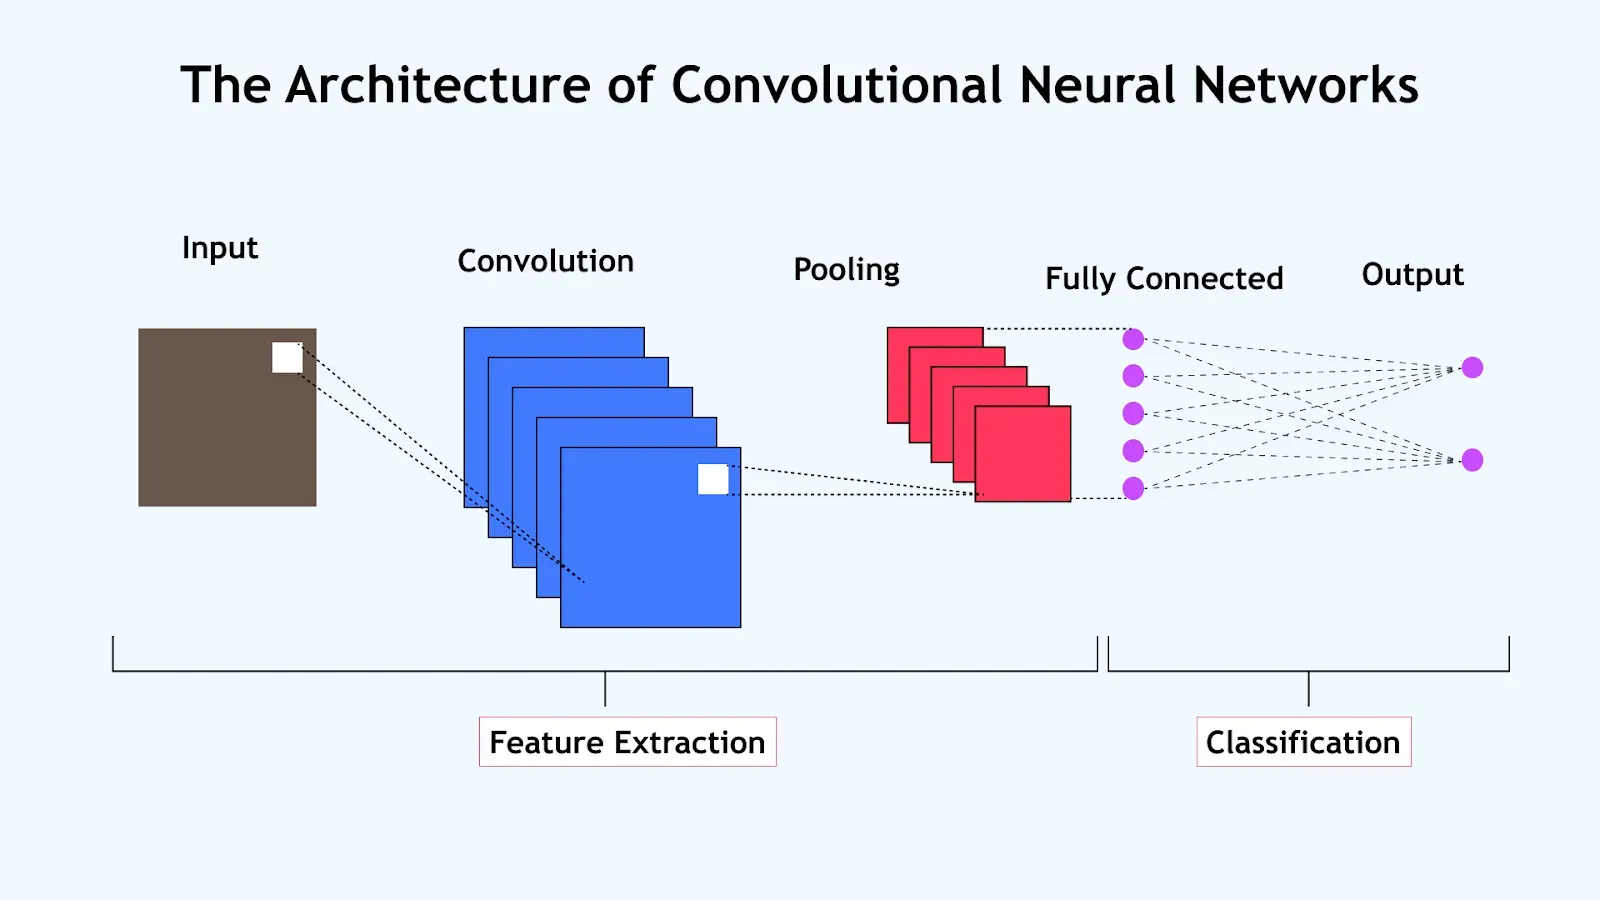
\includegraphics[width=0.85\linewidth]{Images/cnn.png}
    \caption{CNN Architecture}
    \label{fig:CNN Architecture}
\end{figure}

\textbf{Transfer Learning with \gls{vgg16}}

To complement the custom \gls{cnn} and further enhance accuracy, we integrate a
transfer learning approach using the \gls{vgg16} architecture pretrained on the
ImageNet dataset. \gls{vgg16} is a well-established deep network known for its
simplicity and performance in image classification tasks.

In our approach, the \gls{vgg16} base model is used without its top
classification layers. All convolutional layers of \gls{vgg16} are frozen to
retain the pretrained features, which are known to capture generic visual
patterns that are also relevant to medical images.

On top of the \gls{vgg16} base, we add a Global Average Pooling layer followed
by fully connected Dense layers with \gls{relu} activations and Dropout. The
final classification layer uses softmax activation to output probabilities for
each class. This hybrid model combines the general visual understanding of
\gls{vgg16} with task-specific learning layers adapted to brain tumor
detection.

\begin{figure}[H]
    \centering
    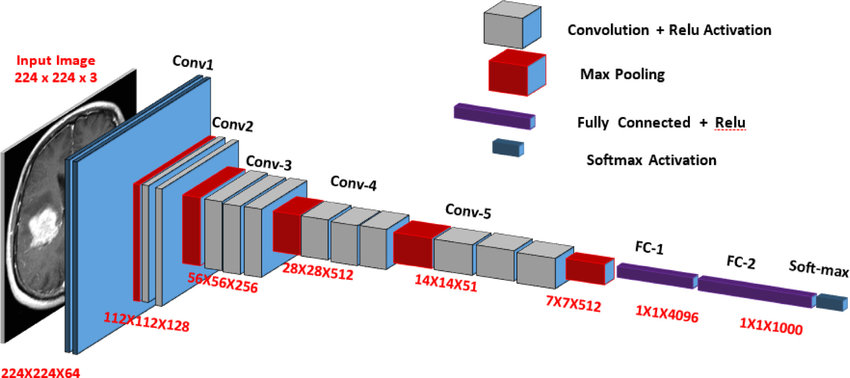
\includegraphics[width=0.85\linewidth]{Images/vgg16.jpg}
    \caption{VGG16 Architecture}
    \label{fig:VGG16 Architecture}
\end{figure}

\textbf{JSON Web Token (JWT) Authentication Algorithm}

The stateless authentication mechanism employs JSON Web Tokens to manage user
sessions and API access control~\cite{jwtio_introduction}. The JWT algorithm
creates digitally signed tokens containing user identity information and access
permissions, typically using Hash-based Message Authentication Code with
\gls{sha256} or \gls{rsa} algorithms for signature
generation~\cite{jwtio_introduction}. Upon successful login, the server
generates a JWT containing the user's ID, email, role, and expiration
timestamp, signing it with a secret key to ensure its integrity and
authenticity. The algorithm enables distributed authentication without
requiring server-side session storage, as each token carries sufficient
information for access verification. Token validation involves signature
verification using the same secret key, expiration time checking, and payload
extraction for user identification. The implementation includes automatic token
refresh mechanisms and secure transmission protocols to maintain session
security while providing seamless user experience across multiple application
components.

\textbf{Bcrypt Password Hashing Algorithm}

The authentication security relies on the bcrypt algorithm for secure password
storage and verification~\cite{geeksforgeeks_bcrypt}. This adaptive hashing
function incorporates a configurable salt parameter that increases
computational complexity and prevents rainbow table attacks. The algorithm
generates unique salt values for each password, combines them with the
plaintext password, and applies multiple rounds of hashing using the Blowfish
cipher~\cite{geeksforgeeks_bcrypt}. The system implements a minimum of 12 salt
rounds, creating a computationally expensive operation that significantly slows
down brute-force attacks while remaining efficient for legitimate
authentication requests. The bcrypt algorithm automatically handles salt
generation and storage within the hash output, enabling seamless password
verification during user login attempts while maintaining resistance against
timing attacks and providing forward security as computational power increases
over time.

